\documentclass{beamer}
%
% Choose how your presentation looks.
%
% For more themes, color themes and font themes, see:
% http://deic.uab.es/~iblanes/beamer_gallery/index_by_theme.html
%
\mode<presentation>
{
  \usetheme{Darmstadt}      % or try Darmstadt, Madrid, Warsaw, ...
  \usecolortheme{default} % or try albatross, beaver, crane, ...
  \usefonttheme{default}  % or try serif, structurebold, ...
  \setbeamertemplate{navigation symbols}{}
  \setbeamertemplate{caption}[numbered]
} 

\usepackage[english]{babel}
\usepackage[utf8x]{inputenc}

\title[Neural Networks]{Neural Networks : An analysis}
\author{Vipul-Anand-Sushant-Nilesh}
\institute{Indian Institute of Technology, Bombay}
\date{March 19, 2014}

\begin{document}

\begin{frame}
  \titlepage
\end{frame}

% Uncomment these lines for an automatically generated outline.
\begin{frame}{Outline}
  \tableofcontents
\end{frame}


\section{Overview}


\subsection{Feedforward Neural Networks \& Backpropagation Algorithm}
\begin{frame}{Feedforward Neural Networks \& Backpropagation Algorithm}
\begin{itemize}
  \item Code Structure
  \item Pseudo Code 
  \item Analysis
\end{itemize}
\end{frame}

\begin{frame}{Code Structure}
We designed the following classes to keep the code modular:
\begin{itemize}
	\item Edge
    \item Neuron
    \item Network\_layer
    \item Neural\_network
\end{itemize}
\end{frame}

\begin{frame}[fragile]{Pseudo Code}
For the backpropagation algorithm :
\begin{verbatim}
Input: NoOfLayers,InputPatterns(Training Data),Learning Rate, Error Threshold, Momentum Factor 
Output: Trained Network 
Network := ConstructNetworkLayers()
InitializeWeights(Network, NoOfLayers)
while(Error != Error Threshold) {
      InputPattern := SelectInputPattern(InputPatterns)
      Output := ForwardPropagate(InputPattern, Network)
      BackwardPropagateError(InputPattern,Output,Network)
      UpdateWeights(InputPattern,Output,Network,Learning Rate,Momentum Factor)
}
Trained Network := Network
Return (Network)
\end{verbatim}

\end{frame}

\begin{frame}{Analysis}
We solved the following problems with the backpropagation algorithm:
\begin{itemize}
	\item NAND
    \item XOR
    \item Five input palindrome
    \item Five input majority
    \item Five input parity 
    \newline
\end{itemize}

We also solved the following application based problems:

\begin{itemize}
	\item Twitter Sentiment Analysis
    \item Flower classification from IRIS data
    \item MONKS classification problems
    \newline
\end{itemize}
\end{frame}

\section{Network Analysis}
    
\begin{frame}[fragile]{Network Analysis}
	\begin{itemize}
    	\item NAND: This training doesnot even requires any hidden layers, as NAND can be even trained on PTA.
   		\item XOR : This requires 1 hidden layer, the hidden layer here computes A.B' and A'.B
        \item 5-Input Palindrome: This also requires hidden layer, one of the neurons at hidden layer computes the equality of outermost inputs and second computes the equality of input(2) and input(4), and the outer most layer uses these inputs to predict if the given input is the palindrome, the middle input(3) is just ignored.
        \item 5 Input Majority: This does not require a hidden layer, and can just be done by a perceptron
        \item 5 Input Parity: In this hidden layer computes, two term at a time xor and then finally computes the xor at the hidden layer.
     \end{itemize}
\end{frame}
\section{Important Questions}
\begin{frame}[fragile]{Important Questions}
	\begin{itemize}
    	\item If we initialze the neural network with equal weights then all neurons will start to behave in the same fashion, so we cannot achieve different functionality by using different neurons, hence the NN loses its purpose.
        \item Saturation in neural network suggests that your NN is a bad health, the neurons which have high weights donot actually function because they get saturated by the smallest of the inputs, so neurons shouldn't be allowed to saturate.
        \item Momentum Factor, helps the FfBbNn to move out of local minima's as it tries to keep the updates in weights moving the direction they were moving at the previous iteration, so in case if the error value becomes low the momentum comes to the rescue.
       \end{itemize}
\end{frame}
\begin{frame}[fragile]{Important Questions}
	\begin{itemize}
        \item Convergence Time of neural network depends on how well have been the initial weights been assigned, or how many layers are present inside the NN. Every data set has a minimu number reuirement in terms of neurons and hidden layer to converge for eg: the Paliandrome requires 1 hidden layer and atleast 2 neurons in it.
        \item Local Minima, many times the neural network error refuses to decrease it happens when the network get stuck in an local minima, at such points tuning to learning rate and momentum factor are required.
    \end{itemize}
\end{frame} 

\section{Graphs}

\subsection{Error vs Iteration Number}
\begin{frame}[fragile]{Graphs}
    	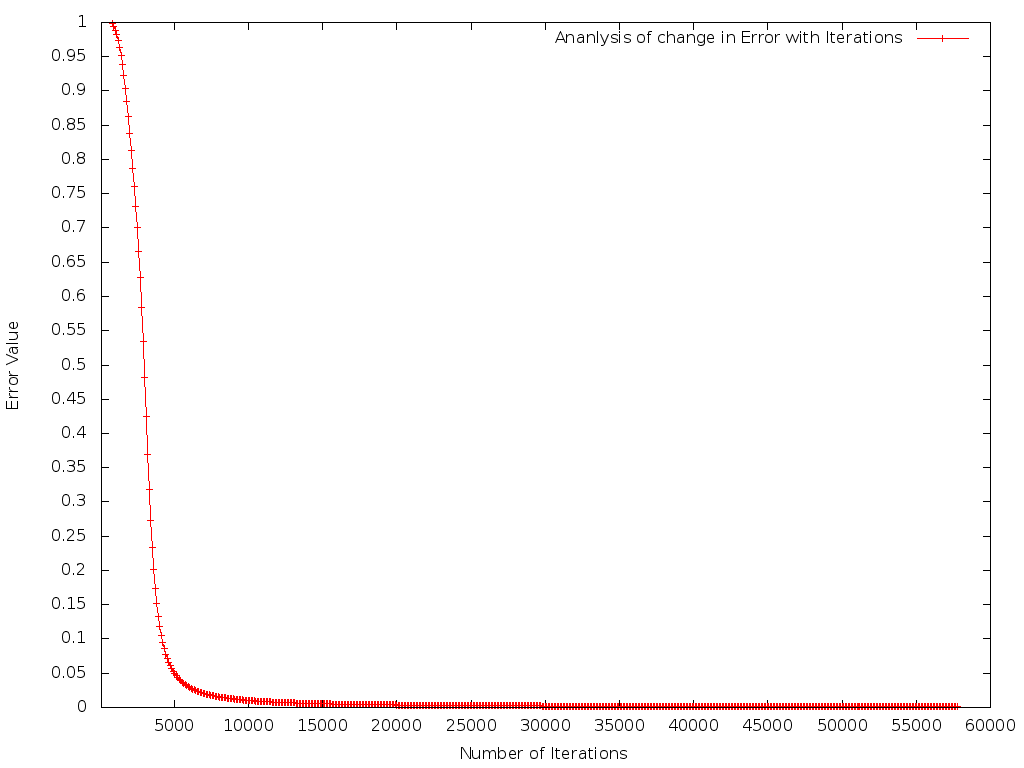
\includegraphics[scale=0.3]{EvsI.png}
\end{frame}

\subsection{Learning Rate vs Iteration Number}
\begin{frame}[fragile]{Graphs}
	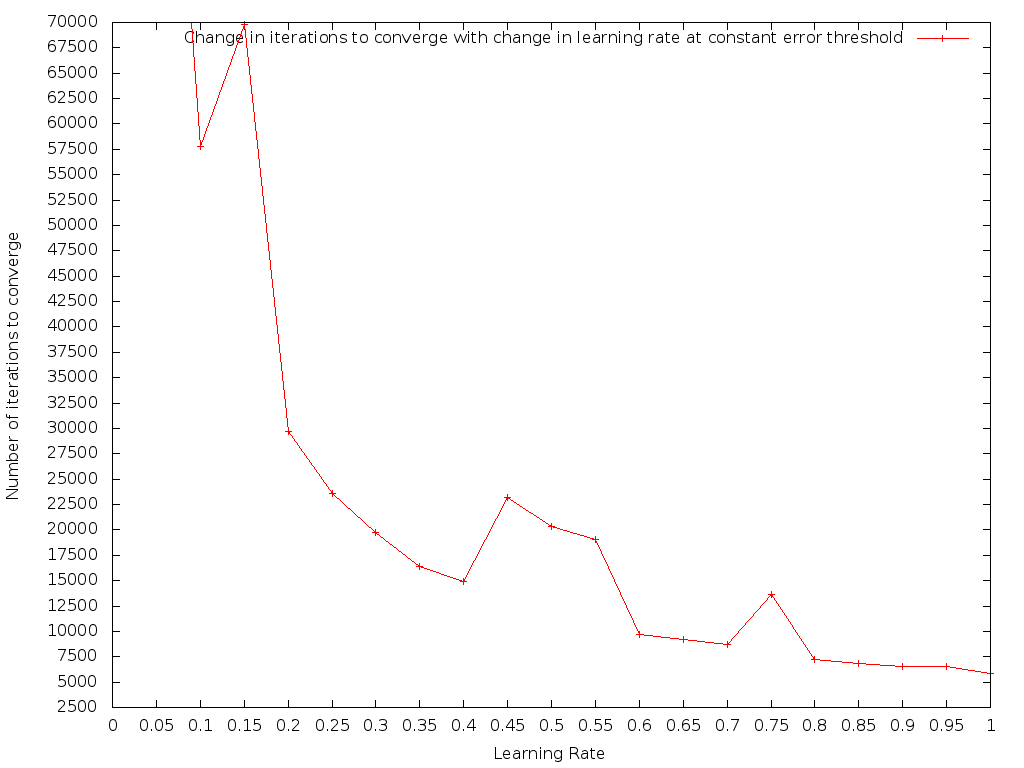
\includegraphics[scale=0.3]{LRvsI.png}
\end{frame}

\subsection{Error vs Iteration Number at different momentum values}
\begin{frame}[fragile]{Graphs}
	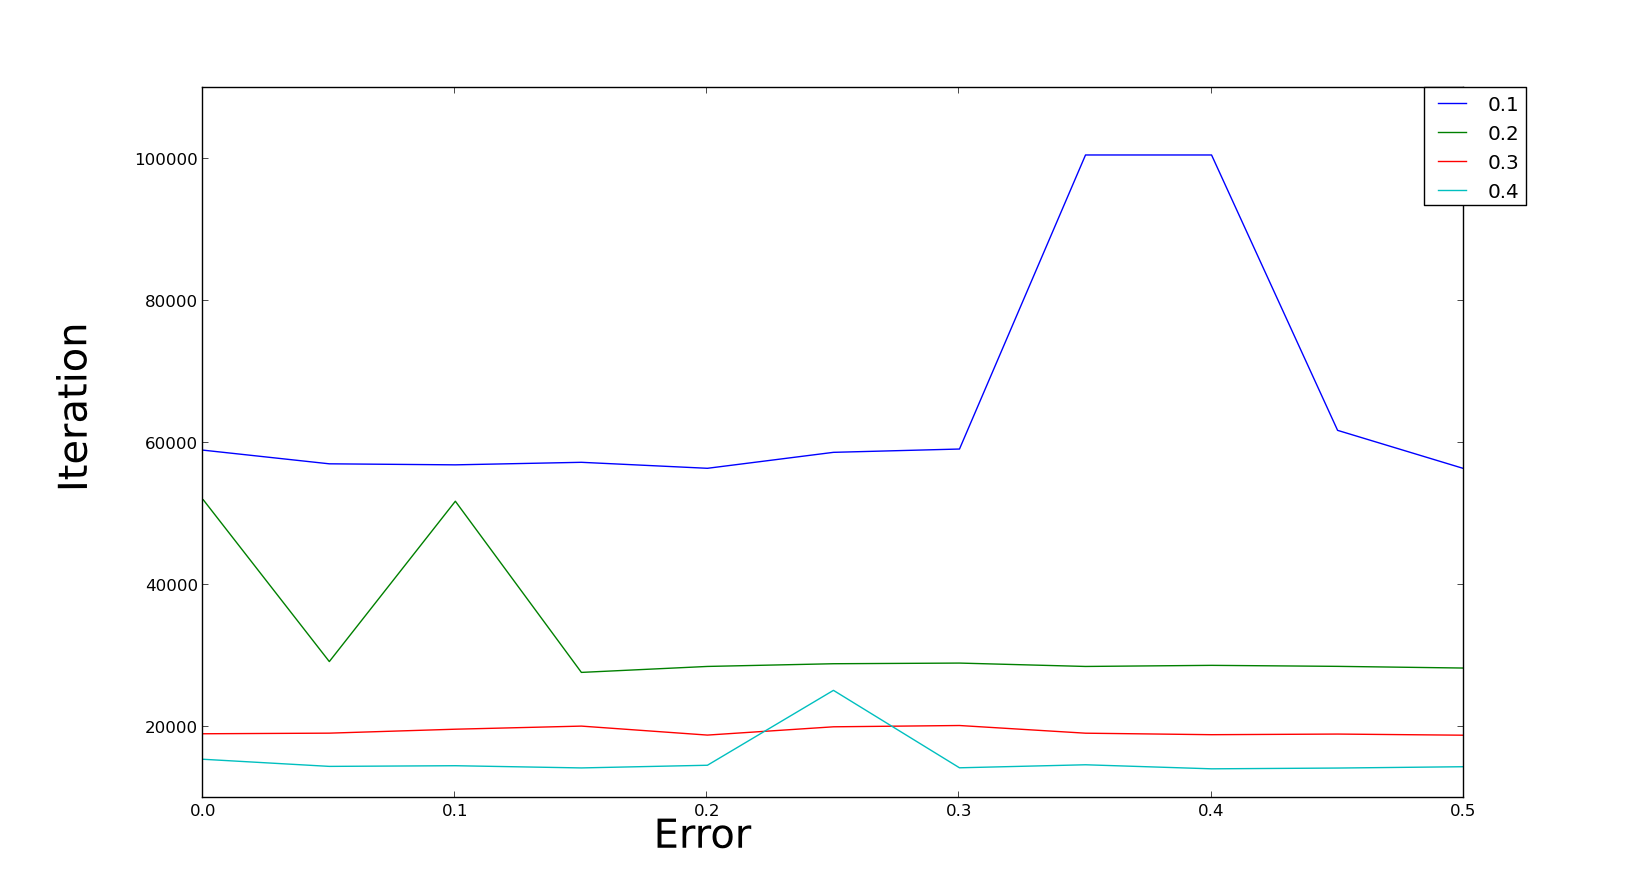
\includegraphics[scale=0.3]{momentum.png}
\end{frame}


\subsection{Convergence of NN}
\begin{frame}[fragile]{Graphs}
	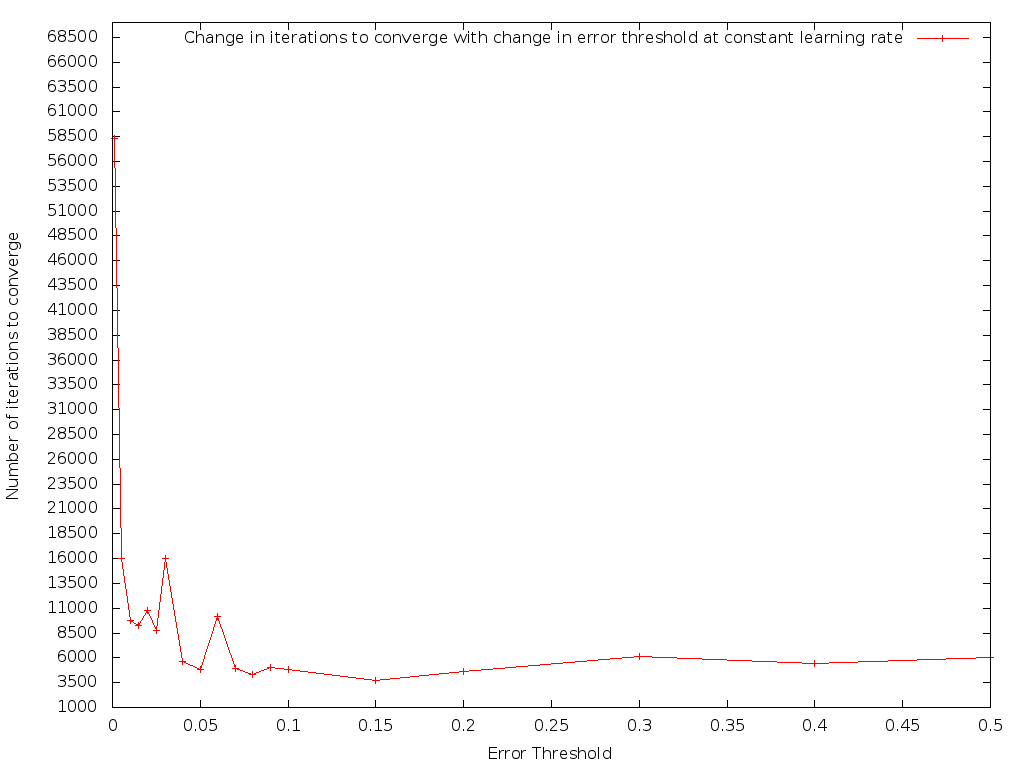
\includegraphics[scale=0.3]{convergence.png}
\end{frame}

\section{Twitter Sentiment Analysis}
\begin{frame}{Twitter Sentiment Analysis}
Extraction of feature vectors:
\begin{itemize}
	\item Preprocessed the tweets to remove hashtags, user names and converted all letters to small case
    \item Removed all stop words (words like 'a', 'the', 'an' and others) which denote no sentiments
    \item Removed all words not starting with an alphabet
    \item Removed words that occurred with the least frequency in the corpus provided
    \item Generated feature vectors of size 530
    \newline
\end{itemize}

The Network:
\begin{itemize}
	\item An input layer with 530 inputs
    \item An output layer with a single neuron giving the output (-1 or 0 or 1)
        
\end{itemize}
\end{frame}

\begin{frame}{Twitter Sentiment Analysis}

\begin{itemize}
	\item No hidden layers!
    \item Squared error threshold kept to 0.5
    \item Learning rate set to 0.1
    \item Momentum kept varying between 0.4-0.8 to avoid getting stuck into local minima
	\newline
\end{itemize}

Results:
\begin{itemize}
	\item Performed 5-fold cross-validation to obtain the mean performance over the input data
    \item Accuracy measured : 83-86 \%
\end{itemize}

\end{frame}

\section{IRIS Data}
\begin{frame}{IRIS Data}
We performed flower classification from the famous IRIS data set.
\newline
The Network:
\begin{itemize}
	\item An input layer with 4 input neurons
    \item An output layer with a single output neuron
    \item One hidden layer with 4 neurons
    \item Learning rate set to 0.3
    \item Momentum set a bit high around 0.8
    \item Squared error threshold kept as 0.8
    \newline
\end{itemize}

Results:
\begin{itemize}
	\item Performed 5-fold cross-validation over input data
    \item Accuracy measured : 90-98 \%
    \item We also performed the classification after removing the petal width column from the input data. Its correlation with petal length was seemingly high!
    \item Accuracy measured without petal width : 90-95 \%
\end{itemize}
\end{frame}

\begin{frame}{MONKS Problems}
We solved all the three MONKS problems.\newline
MONKS-1 Analysis
The Network:
\begin{itemize}
	\item An input layer with 6 inputs
    \item An output layer with a single output neuron
    \item One hidden layer with 3 neurons
    \item Learning rate set to 0.1
    \item Momentum set a bit high around 0.9
    \item Squared error threshold kept as 0.9
    \newline 
\end{itemize}
Results:
\begin{itemize}
	\item Performed 5-fold cross-validation over input data
    \item Accuracy measured : 98-100 \%    
\end{itemize}
\end{frame}

\begin{frame}{MONKS Problems}
MONKS-2 Analysis\newline
The Network:
\begin{itemize}
	\item An input layer with 6 inputs
    \item An output layer with a single output neuron
    \item Three hidden layer with 12, 6 and 2 neurons respectively
    \item Learning rate set to 0.1
    \item Momentum set a bit high around 0.9
    \item Squared error threshold kept as 0.9
    \newline 
\end{itemize}
Results:
\begin{itemize}
	\item Performed 5-fold cross-validation over input data
    \item Accuracy measured : 98-100 \%    
\end{itemize}

\end{frame}
\begin{frame}{MONKS Problems}
MONKS-3 Analysis\newline
The Network:
\begin{itemize}
	\item An input layer with 6 inputs
    \item An output layer with a single output neuron
    \item One hidden layer with 3 neurons
    \item Learning rate set to 0.1
    \item Momentum set a bit high around 0.9
    \item Squared error threshold kept as 0.5
    \newline 
\end{itemize}
Results:
\begin{itemize}
	\item Performed 5-fold cross-validation over input data
    \item Accuracy measured : 98-100 \%    
\end{itemize}

\end{frame}

\begin{frame}{Analysis}
Graphical analysis to study the properties of the neural network during the training phase:

\end{frame}

%\begin{figure}
%\includegraphics[width=\textwidth]{}
%\caption{\label{fig:your-figure}Caption goes here.}
%\end{figure}


\vskip 1cm

% Commands to include a figure:
%\begin{figure}
%\includegraphics[width=\textwidth]{your-figure's-file-name}
%\caption{\label{fig:your-figure}Caption goes here.}
%\end{figure}



\end{document}
